\documentclass[12pt, a4paper]{article}
\usepackage[utf8]{inputenc}
\usepackage{polski}
\usepackage{amssymb}
\usepackage{amsmath}
\usepackage{fancyhdr}
\usepackage{multicol}
\usepackage{graphicx}
\setlength{\voffset}{-0.75in}
\setlength{\headsep}{5pt}
\setlength{\hoffset}{-40pt}
\setlength{\textwidth}{500pt}
\setlength{\textheight}{770pt}
\setlength{\parindent}{0em}

\begin{document}

Rozważamy cztery równania różniczkowe cząstkowe.\\

Równanie transportu
\begin{equation}
\frac{\partial u}{\partial t}+\frac{\partial u}{\partial x}=0, 0\leqslant x\leqslant10, t\geqslant0.
\end{equation}
\vspace{0.5cm}

Nielepkie równanie Burgersa
\begin{equation}
\frac{\partial u}{\partial t}+u\frac{\partial u}{\partial x}=0, 0\leqslant x\leqslant10, t\geqslant0.
\end{equation}
\vspace{0.5cm}

Równanie ciepła
\begin{equation}
\frac{\partial u}{\partial t}-\beta\frac{\partial^{2} u}{\partial x^{2}}=0, 0\leqslant x\leqslant10, t\geqslant0, \beta>0.
\end{equation}
\vspace{0.5cm}

Równanie Burgersa (nieliniowe, paraboliczne)
\begin{equation}
\frac{\partial u}{\partial t}+u\frac{\partial u}{\partial x}-\beta\frac{\partial^{2} u}{\partial x^{2}}=0, 0\leqslant x\leqslant10, t\geqslant0, \beta>0.
\end{equation}
Dla wszystkich czterech równań:\\
\begin{itemize}
\item $t$ - zmienna niezależna interpretowana jako czas,
\item $x$ - zmienna niezależna interpretowana jako położenie,
\item $u(x,t)$ - zmienna zależna interpretowana jako prędkość płynu,
\item $\beta$ - stały parametr interpretowany jako lepkość płynu.
\end{itemize}
\vspace{0.5cm}

Naszym celem jest wykorzystanie metod różnic skończonych w celu znalezienia przybliżonych\\
wartości $u(x,t)$ rozwiązania wszystkich równań.\\
Najpierw określmy krok przestrzenny $h$ oraz krok czasowy $k$. Niech
\begin{equation}
\begin{split}
& u_{i,j}=u(x_{i},t_{j})=u(i\cdot h,j\cdot k),\\
& h=0.1, k=0.005, i\in[0,M-1], j\in[0,N-1], M,N\in\mathbb{N}.
\end{split}
\end{equation}

Wtedy niech warunek początkowy wszystkich równań (funkcja Gaussa)
\begin{equation}
u_{i,0}=e^{-(x_{i}-x_{mid})^{2}}, x_{mid}=\frac{(M - 1) \cdot h}{2}=5.
\end{equation}

Oraz niech warunki brzegowe wszystkich równań
\begin{equation}
u_{0,j}=u_{M-1,j}=0.
\end{equation}

Niech 
\begin{equation}
\beta<\frac{h^{2}}{2k}\land\beta=0.99,
\end{equation}
w celu uzyskania stabilności rozwiązań.
\newpage

Wtedy stosując metodę Eulera:\\
dla równania transportu
\begin{equation}
\begin{split}
& \frac{1}{k}(u_{i,j+1}-u_{i,j})+\frac{1}{2h}(u_{i+1,j}-u_{i-1,j})=0,\\
& u_{i,j+1}=u_{i,j}-\frac{k}{2h}(u_{i+1,j}-u_{i-1,j}),
\end{split}
\end{equation}
\begin{figure}[h]
\caption{Równanie transportu, metoda Eulera}
\centering
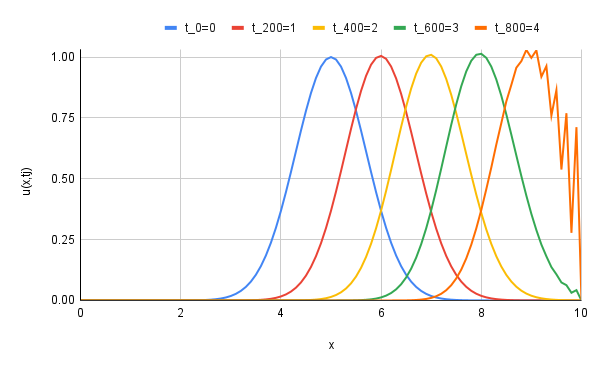
\includegraphics[width=0.75\textwidth]{0.png}
\end{figure}

dla nielepkiego równania Burgersa
\begin{equation}
\begin{split}
& \frac{1}{k}(u_{i,j+1}-u_{i,j})+\frac{1}{4h}(u_{i+1,j}^{2}-u_{i-1,j}^{2})=0,\\
& u_{i,j+1}=u_{i,j}-\frac{k}{4h}(u_{i+1,j}^{2}-u_{i-1,j}^{2}),
\end{split}
\end{equation}
\begin{figure}[h]
\caption{Nielepkie równanie Burgersa, metoda Eulera}
\centering
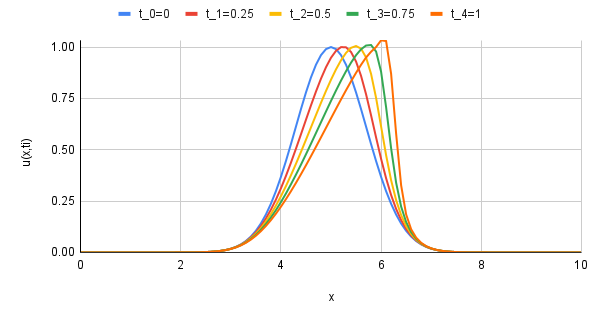
\includegraphics[width=0.65\textwidth]{1.png}
\end{figure}
\newpage

dla równania ciepła
\begin{equation}
\begin{split}
& \frac{1}{k}(u_{i,j+1}-u_{i,j})-\frac{\beta}{h^{2}}(u_{i+1,j}-2u_{i,j}+u_{i-1,j})=0,\\
& u_{i,j+1}=u_{i,j}+\frac{\beta k}{h^{2}}(u_{i+1,j}-2u_{i,j}+u_{i-1,j}),
\end{split}
\end{equation}
\begin{figure}[h]
\caption{Równanie ciepła, metoda Eulera}
\centering
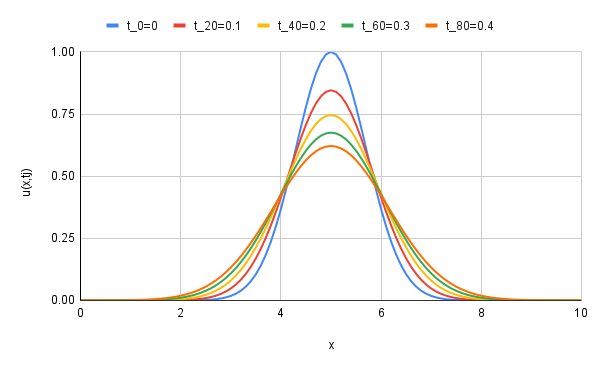
\includegraphics[width=0.65\textwidth]{2.png}
\end{figure}

dla równania Burgersa
\begin{equation}
\begin{split}
& \frac{1}{k}(u_{i,j+1}-u_{i,j})+\frac{1}{4h}(u_{i+1,j}^{2}-u_{i-1,j}^{2})-\frac{\beta}{h^{2}}(u_{i+1,j}-2u_{i,j}+u_{i-1,j})=0,\\
& u_{i,j+1}=u_{i,j}-\frac{k}{4h}(u_{i+1,j}^{2}-u_{i-1,j}^{2})+\frac{\beta k}{h^{2}}(u_{i+1,j}-2u_{i,j}+u_{i-1,j}).
\end{split}
\end{equation}
\begin{figure}[h]
\caption{Równanie Burgersa, metoda Eulera}
\centering
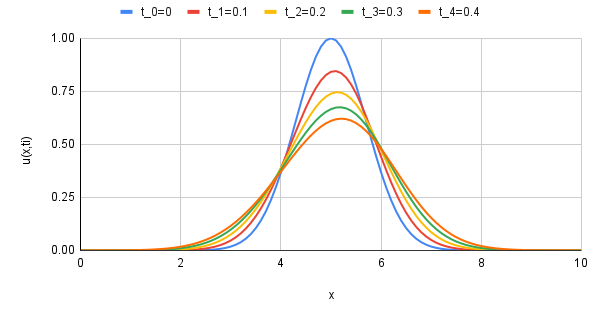
\includegraphics[width=0.65\textwidth]{3}
\end{figure}
\newpage

Stosując metodę Rungego-Kutty drugiego rzędu:\\
dla równania transportu
\begin{equation}
\begin{split}
& v_{i,j+1}=u_{i,j}-\frac{k}{4h}(u_{i+1,j}-u_{i-1,j}),\\
& u_{i,j+1}=u_{i,j}-\frac{k}{2h}(v_{i+1,j+1}-v_{i-1,j+1}),
\end{split}
\end{equation}
\begin{figure}[h]
\caption{Równanie transportu, metoda RK2}
\centering
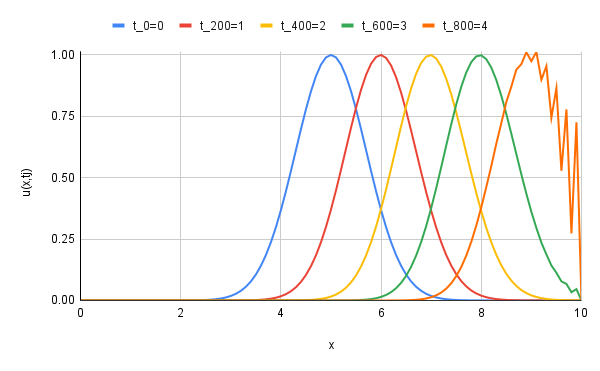
\includegraphics[width=0.65\textwidth]{4}
\end{figure}

dla nielepkiego równania Burgersa
\begin{equation}
\begin{split}
& v_{i,j+1}=u_{i,j}-\frac{k}{8h}(u_{i+1,j}^{2}-u_{i-1,j}^{2}),\\
& u_{i,j+1}=u_{i,j}-\frac{k}{4h}(v_{i+1,j+1}^{2}-v_{i-1,j+1}^{2}),
\end{split}
\end{equation}
\begin{figure}[h]
\caption{Nielepkie równanie Burgersa, metoda RK2}
\centering
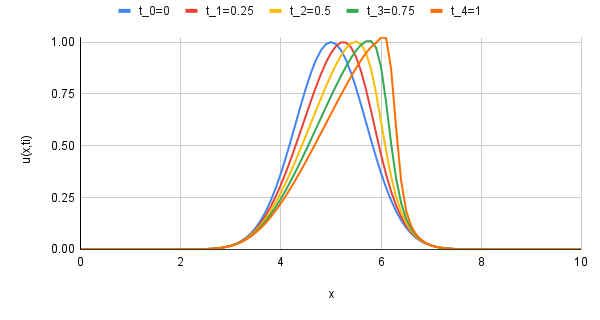
\includegraphics[width=0.65\textwidth]{5}
\end{figure}
\newpage
\newpage

dla równania ciepła
\begin{equation}
\begin{split}
& v_{i,j+1}=u_{i,j}+\frac{\beta k}{2h^{2}}(u_{i+1,j}-2u_{i,j}+u_{i-1,j}),\\
& u_{i,j+1}=u_{i,j}+\frac{\beta k}{h^{2}}(v_{i+1,j+1}-2v_{i,j+1}+v_{i-1,j+1}),
\end{split}
\end{equation}
\begin{figure}[h]
\caption{Równanie ciepła, metoda RK2}
\centering
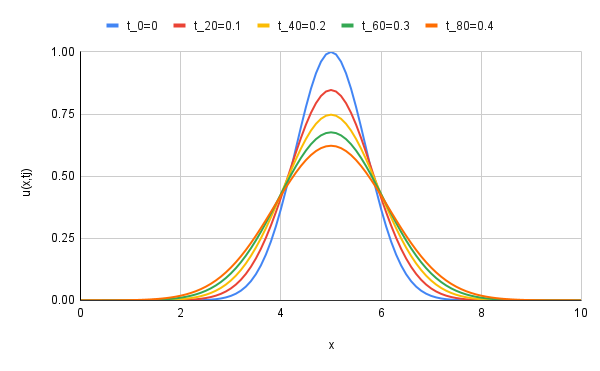
\includegraphics[width=0.75\textwidth]{6}
\end{figure}

dla równania Burgersa
\begin{equation}
\begin{split}
& v_{i,j+1}=u_{i,j}-\frac{k}{8h}(u_{i+1,j}^{2}-u_{i-1,j}^{2})+\frac{\beta k}{2h^{2}}(u_{i+1,j}-2u_{i,j}+u_{i-1,j}),\\
& u_{i,j+1}=u_{i,j}-\frac{k}{4h}(v_{i+1,j+1}^{2}-v_{i-1,j+1}^{2})+\frac{\beta k}{h^{2}}(v_{i+1,j+1}-2v_{i,j+1}+v_{i-1,j+1}).
\end{split}
\end{equation}
\begin{figure}[h]
\caption{Równanie Burgersa, metoda RK2}
\centering
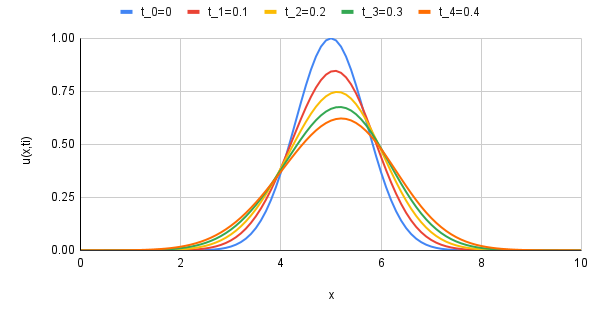
\includegraphics[width=0.65\textwidth]{7}
\end{figure}

\newpage
Stosując metodę niejawną:\\
dla równania ciepła
\begin{equation}
\begin{split}
& \frac{1}{k}(u_{i,j}-u_{i,j-1})-\frac{\beta}{h^{2}}(u_{i+1,j}-2u_{i,j}+u_{i-1,j})=0,\\
& u_{i,j-1}=-\frac{\beta k}{h^{2}}u_{i-1,j}+(1+2\frac{\beta k}{h^{2}})u_{i,j}-\frac{\beta k}{h^{2}}u_{i+1,j},
\end{split}
\end{equation}
\begin{center}
$A=
\begin{bmatrix}
1+2s & -s & 0 & \cdots & 0\\
-s & 1+2s & -s & \cdots & 0\\
0 & -s & 1+2s & \cdots & 0\\
\cdots & \cdots & \cdots & \cdots & \cdots\\
0 & 0 & 0 & \cdots & 1+2s\\
\end{bmatrix}$
$, s=\frac{\beta k}{h^{2}}$,
\end{center}
\begin{equation}
u_{i,j}=A^{-1}u_{i,j-1},
\end{equation}
\begin{figure}[h]
\caption{Równanie ciepła, metoda niejawna}
\centering
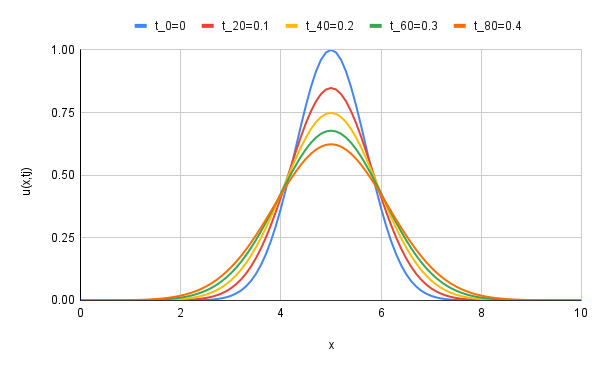
\includegraphics[width=0.65\textwidth]{8}
\end{figure}
\newpage

dla równania Burgersa
\begin{equation}
\begin{split}
& \frac{1}{k}(u_{i,j}-u_{i,j-1})+\frac{1}{4h}(u_{i+1,j-1}^{2}-u_{i-1,j-1}^{2})-\frac{\beta}{h^{2}}(u_{i+1,j}-2u_{i,j}+u_{i-1,j})=0,\\
& u_{i,j-1}-\frac{k}{4h}(u_{i+1,j-1}^{2}-u_{i-1,j-1}^{2})=-\frac{\beta k}{h^{2}}u_{i-1,j}+(1+2\frac{\beta k}{h^{2}})u_{i,j}-\frac{\beta k}{h^{2}}u_{i+1,j},
\end{split}
\end{equation}
\begin{center}
$A=
\begin{bmatrix}
1+2s & -s & 0 & \cdots & 0\\
-s & 1+2s & -s & \cdots & 0\\
0 & -s & 1+2s & \cdots & 0\\
\cdots & \cdots & \cdots & \cdots & \cdots\\
0 & 0 & 0 & \cdots & 1+2s\\
\end{bmatrix}$
$,s=\frac{\beta k}{h^{2}}$,
\end{center}
\begin{equation}
u_{i,j}=A^{-1}(u_{i,j-1}-\frac{k}{4h}(u_{i+1,j-1}^{2}-u_{i-1,j-1}^{2})).
\end{equation}
\begin{figure}[h]
\caption{Równanie Burgersa, metoda niejawna}
\centering
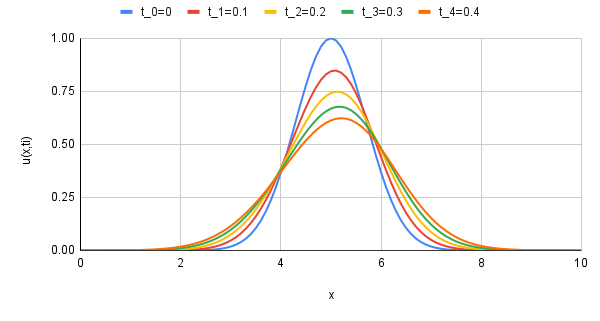
\includegraphics[width=0.65\textwidth]{9}
\end{figure}
\newline
Algorytm, który realizuje opisaną metodę niejawną korzysta z procedury tri rozwiązującej układ równań o macierzy trójprzekątniowej. Metoda tri korzysta ze szczególnego przypadku eliminacji Gaussa w czasie $O(n)$, zamiast czasu $O(n^3)$ dla normalnego przypadku, co ogromnie przyspiesza znajdowanie rozwiązań. Mogliśmy zasotosować tę metodę ponieważ stałe wartości na głównej przekątnej były dodatnie oraz większe od wartości na górnej oraz dolnej przekątnej. 
\newpage

Uzyskaliśmy prawie identyczne wyniki za pomocą użycia metody Eulera, RK2 i niejawnej. Nie mogliśmy skorzystać z metody niejawnej dla równania transportu, ani dla nielepkiego równania Burgersa, ponieważ wymaga ona użycia macierzy kwadratowej (M=N), a dla tych równań ta równość nie zachodziła, ponieważ nie chcieliśmy ograniczać $t$ aż tak bardzo.\\

Dla równania transportu oraz nielepkiego równania Burgersa, jeśli $t$ przekroczy odpowiednią wartość, to przybliżone wartości $u$ zaczynają bardzo mocno odbiegać od rzeczywistych (dla równania transportu $t>3$, dla nielepkiego równania Burgersa, $t>1$).\\

Dla równania transportu, kolejne przesunięcia w czasie $t_{j}$ powodują uzyskanie maksmimum $u=1$ w kolejnych przesunięciach w przestrzeni $x_{i}$.  Funkcja Gaussa zostaje jedynie przesunięta w prawo.  Zobrazowna zostaje liniowość.\\

Dla nielepkiego równania Burgera, kolejne przesunięcia w czasie $t_{j}$ powodują uzyskanie maksimum $u=1$ w kolejnych przesunięciach w przestrzeni $x_{i}$. Funkcja Gaussa nie zostaje jedynie przesunięta w prawo, tylko wolniej rośnie przed osiągnieciem maksimum i szybciej maleje po osiągnięciu maksimum. Zobrazowna zostaje nieliniowość i pokazany zostaje efekt "fali uderzeniowej".\\

Dla równania ciepła, kolejne przesunięcia w czasie $t_{j}$ powodują zmniejszenie maksimum funkcji Gaussa. Maksimum $u<1$ jedynie maleje w tym samym punkcie w przestrzeni $x_{mid}=5$ dla kolejnych czasów $t_{j}$.\\ 

Dla równania Burgersa, kolejne przesunięcia w czasie $t_{j}$ powodują zmniejszenie maksimum funkcji Gaussa oraz powodują efekt "fali uderzeniowej". Maksimum $u<1$ maleje i przesuwa się w przestrzeni $x_{i}$ dla kolejnych czasów $t_{j}$.\\

Zwiększanie współczynnika $\beta$ powoduje zmniejszenie maksimum $u(x,t)$ dla kolejnych czasów $t_{j}$. Dzieje się tak do około $\beta\leqslant1.2$, po czym dla  $\beta>1.2$ rozwiązanie staje się całkowicie niepoprawne.\\
\begin{figure}[h]
\caption{Równanie Burgersa, metoda Eulera, $\beta$=1.3}
\centering
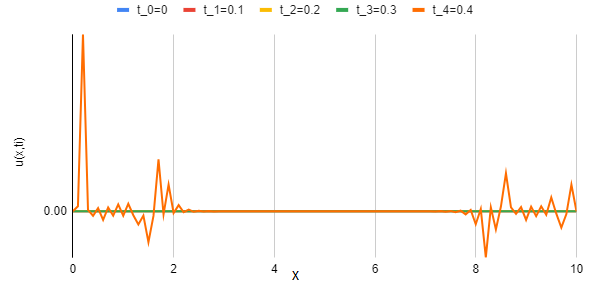
\includegraphics[width=0.65\textwidth]{10}
\end{figure}

Program komputerowy w języku C++ wyznaczający powyższe rozwiązania został dołączony w Dodatku A.
\end{document}